% DO NOT COMPILE THIS FILE DIRECTLY!
% This is included by the other .tex files.

\begin{frame}[t,plain]
\titlepage
\end{frame}

\begin{frame}
	\frametitle{Plan for this session}
	\begin{itemize}
		\item Explanation of the CSIRT use case for information sharing and what CIRCL does
        \item Building an information sharing community and best practices\footnote{We published the complete guidelines in \url{https://www.x-isac.org/assets/images/guidelines_to_set-up_an_ISAC.pdf}}
	\end{itemize}
\end{frame}

\begin{frame}
\frametitle{Communities operated by CIRCL}
\begin{itemize}
        \item As a CSIRT, CIRCL operates a wide range of communities
        \item We use it as an {\bf internal tool} to cover various day-to-day activities
        \item Whilst being the main driving force behind the development, we're also one of the largest consumers
	\item Different communities have different needs and restrictions
\end{itemize}
\end{frame}

\begin{frame}
\frametitle{Communities operated by CIRCL}
\begin{itemize}
        \item Private sector community
	\begin{itemize}
		\item Our largest sharing community
		\item Over {\bf 1000 organisations}
		\item {\bf ~2700 users}
		\item Functions as a central hub for a lot of sharing communities
		\item Private organisations, Researchers, Various SoCs, some CSIRTs, etc
	\end{itemize}
	\item CSIRT community
	\begin{itemize}
		\item Tighter community
		\item National CSIRTs, connections to international organisations, etc
	\end{itemize}
\end{itemize}
\end{frame}

\begin{frame}
\frametitle{Communities operated by CIRCL}
\begin{itemize}
	\item Financial sector community
	\begin{itemize}
		\item Banks, payment processors, etc.
		\item Sharing of {\bf mule accounts} and {\bf non-cyber threat infomartion}
	\end{itemize}
    \item X-ISAC\footnote{\url{https://www.x-isac.org/}}
	\begin{itemize}
		\item {\bf Bridging the gap} between the various sectorial and geographical ISACs
		\item New, but ambitious initiative
		\item Goal is to {\bf bootstrap the cross-sectorial sharing} along with building the infrastructure to enable sharing when needed
	\end{itemize}
\end{itemize}
\end{frame}

\begin{frame}
\frametitle{Communities operated by CIRCL}
\begin{itemize}
        \item the ATT\&CK EU community\footnote{\url{https://www.attack-community.org/}}
	\begin{itemize}
		\item Work on attacker modelling
		\item With the assistance of MITRE themselves
		\item Unique opportunity to {\bf standardise on TTPs}
		\item Looking for organisations that want to get involved!
	\end{itemize}
\end{itemize}
\end{frame}

\begin{frame}
\frametitle{Communities supported by CIRCL}
\begin{itemize}
	\item FIRST.org's MISP community
	\item Telecom and Mobile operators' community
	\item Various ad-hoc communities for exercises for example
	\begin{itemize}
		\item The ENISA exercise for example
	\end{itemize}
\end{itemize}
\end{frame}

\begin{frame}
\frametitle{Sharing Scenarios in MISP}
\begin{itemize}
	\item Sharing can happen for {\bf many different reasons}. Let's see what we believe are the typical CSIRT scenarios
        \item We can generally split these activities into 4 main groups when we're talking about traditional CSIRT tasks:
	\begin{itemize}
		\item Core services
		\item Proactive services
		\item Advanced services
		\item Sharing communities managed by CSIRTs for various tasks
	\end{itemize}
\end{itemize}
\end{frame}

\begin{frame}
\frametitle{CSIRT core services}
\begin{itemize}
	\item Incident response
	\begin{itemize}
		\item {\bf Internal storage} of incident response data
		\item Sharing of indicators {\bf derived from incident response}
		\item {\bf Correlating data} derived and using the built in analysis tools
		\item {\bf Enrichment} services
		\item {\bf Collaboration} with affected parties via MISP during IR
		\item {\bf Co-ordination} and collaboration
		\item {\bf Takedown} requests
	\end{itemize}
	\item Alerting of information leaks (integration with {\bf AIL}\footnote{\url{https://github.com/CIRCL/AIL-framework}})
\end{itemize}
\end{frame}

\begin{frame}
\frametitle{CSIRT proactive services}
\begin{itemize}
	\item {\bf Contextualising} both internal and external data
	\item {\bf Collection} and {\bf dissimination} of data from various sources (including OSINT)
	\item Storing, correlating and sharing own manual research ({\bf reversing, behavioural analysis})
	\item Aggregating automated collection ({\bf sandboxing, honeypots, spamtraps, sensors})
	\begin{itemize}
		\item MISP allows for the creation of {\bf internal MISP "clouds"}
		\item Store {\bf large specialised datasets} (for example honeypot data)
		\item MISP has {\bf interactions with} a large set of such {\bf tools} (Cuckoo, Mail2MISP, etc)
	\end{itemize}
	\item {\bf Situational awareness} tools to monitor trends and adversary TTPs within my sector/geographical region (MISP-dashboard, built in statistics)
\end{itemize}
\end{frame}

\begin{frame}
\frametitle{CSIRT proactive services - MISP dashboard}
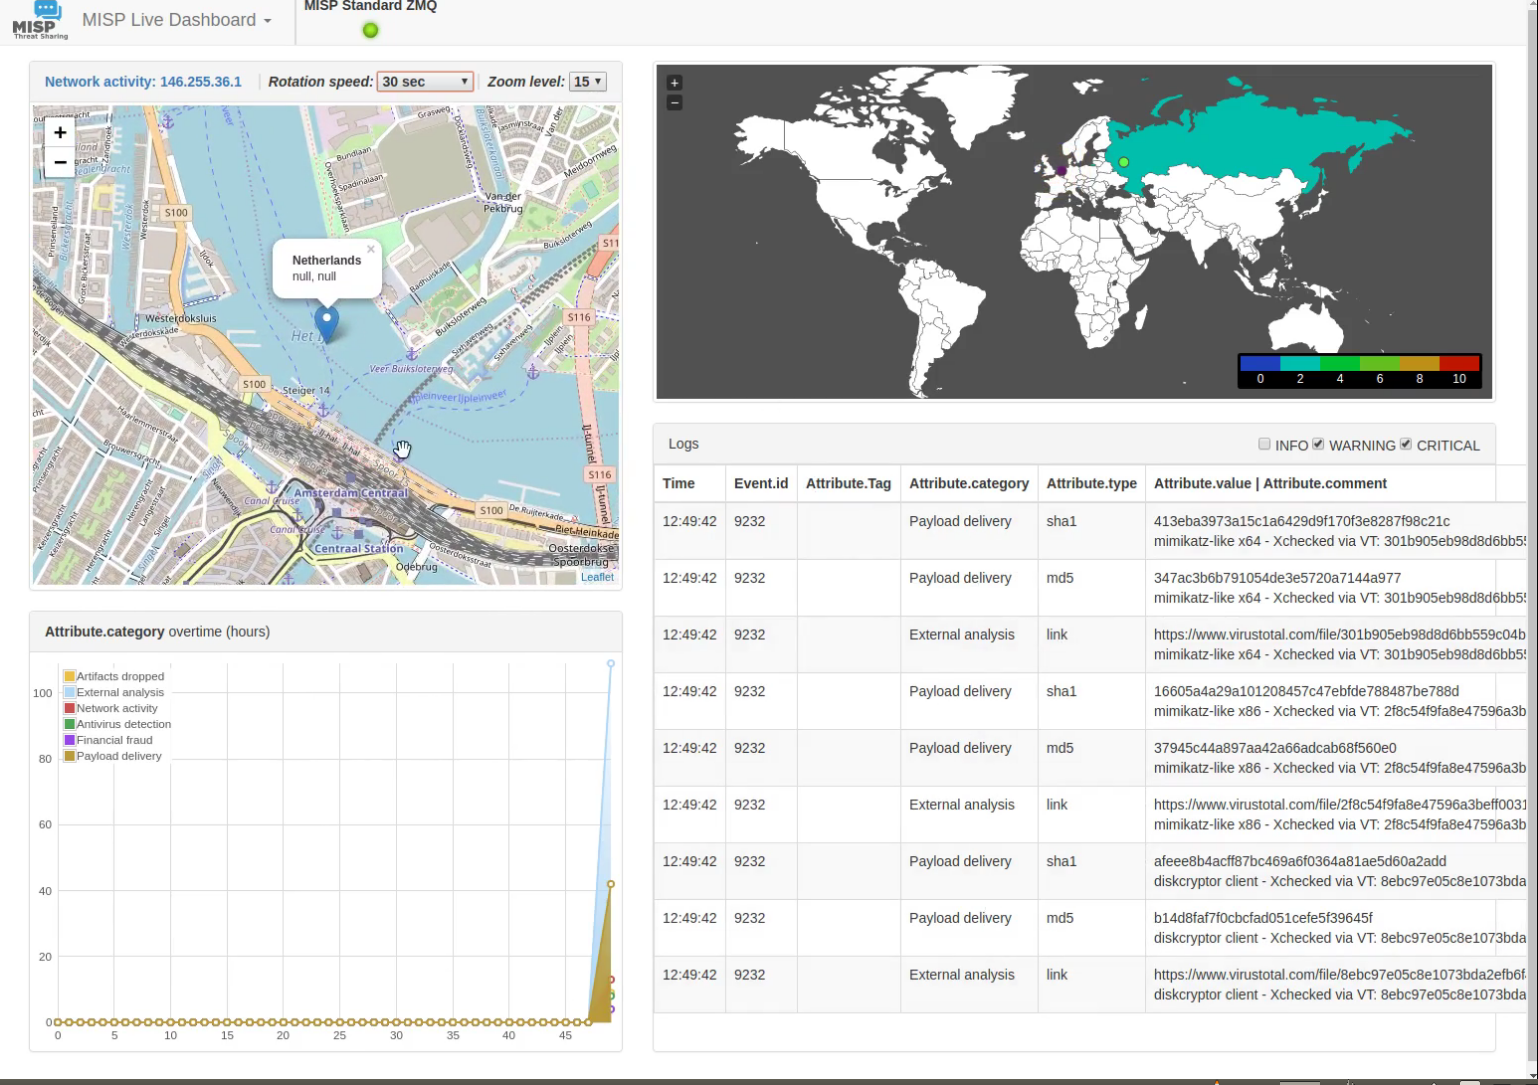
\includegraphics[scale=0.18]{screenshots/dashboard-live.png}
\end{frame}

\begin{frame}
\frametitle{CSIRT proactive services - MISP dashboard}
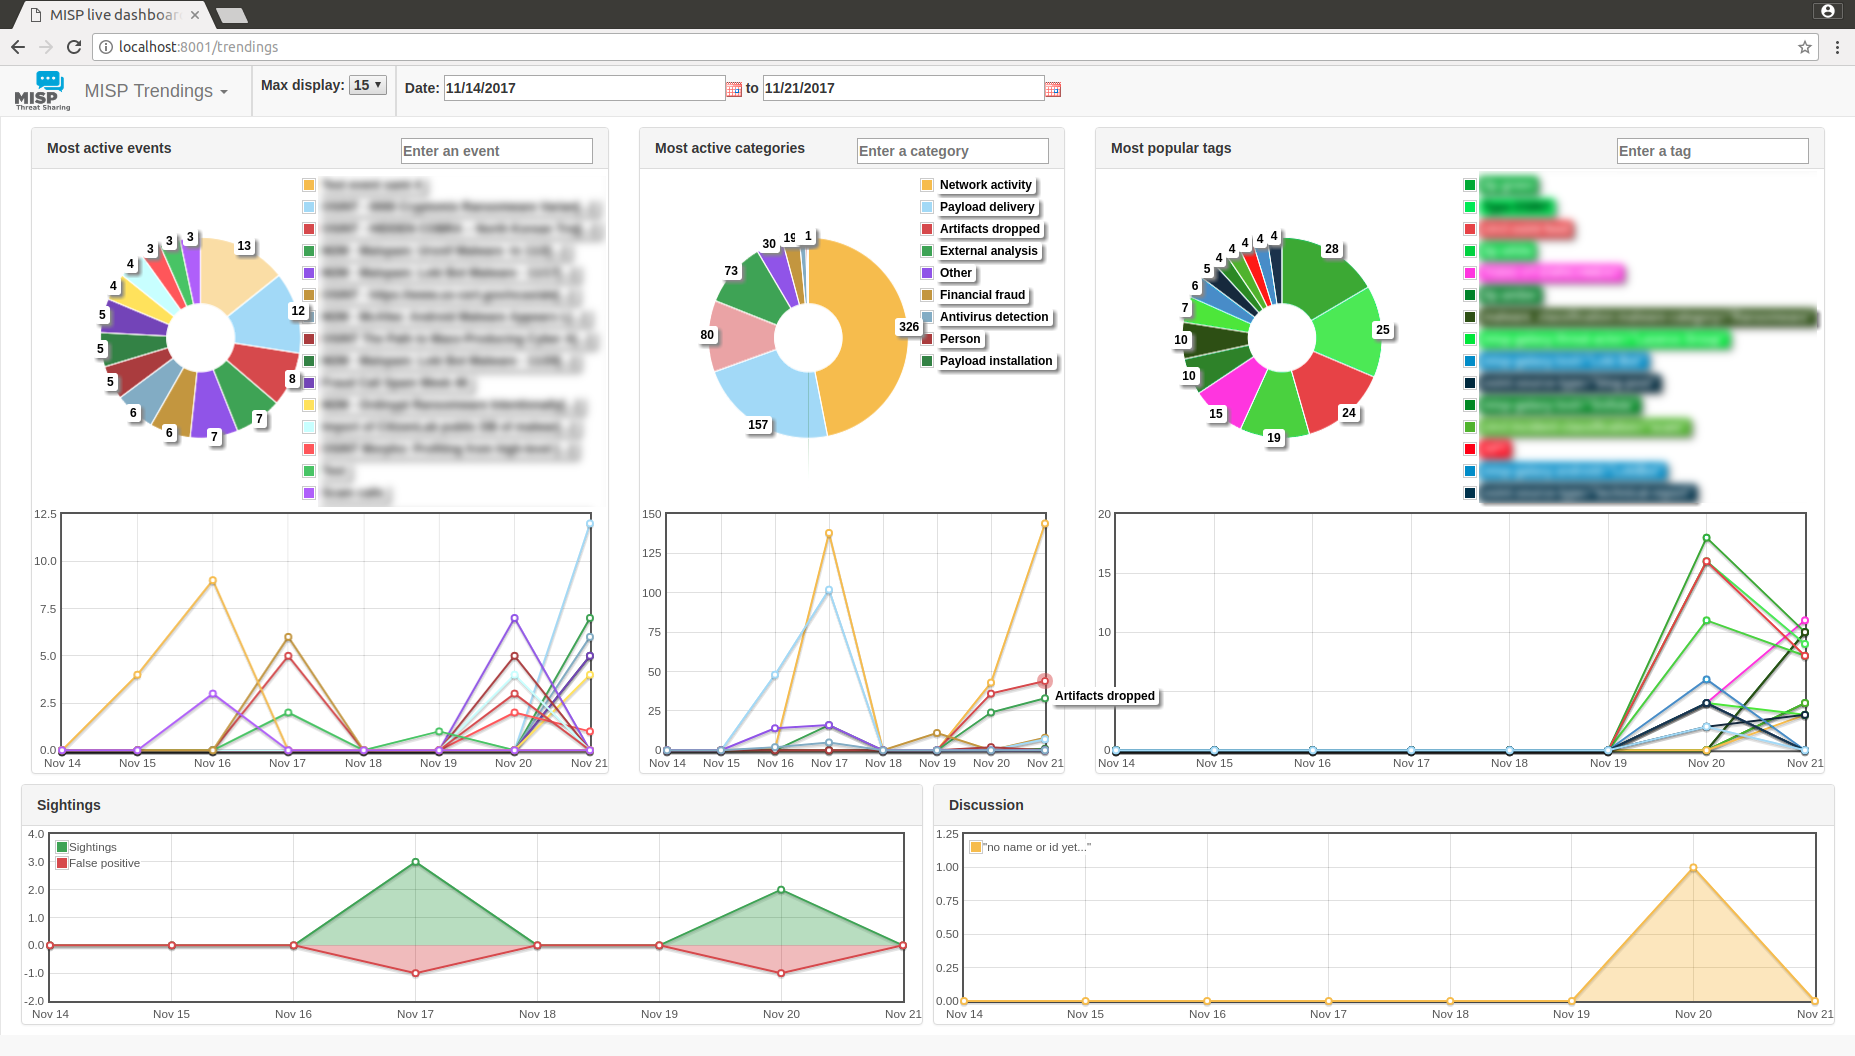
\includegraphics[scale=0.18]{screenshots/dashboard-trendings.png}
\end{frame}

\begin{frame}
\frametitle{CSIRT advanced services}
\begin{itemize}
	\item Supporting {\bf forensic analysts}
	\item Collaboration with {\bf law enforcement}
	\item {\bf Vulnerability} information sharing
	\begin{itemize}
		\item {\bf Notifications} to the constituency about relevant vulnerabilities
		\item {\bf Co-ordinating} with vendors for notifications (*)
		\item Internal / closed community sharing of pentest results
		\item We're planning on starting a series of hackathons to find
	\end{itemize}
\end{itemize}
\end{frame}


\begin{frame}
\frametitle{CSIRTs' management of sharing communities for constituent actions:}
\begin{itemize}
	\item {\bf Reporting} non-identifying information about incidents (such as outlined in NISD)
	\item {\bf Seeking} and engaging in {\bf collaboration} with CSIRT or other parties during an incident
	\item Pre-sharing information to {\bf request for help} / additional information from the community
	\item {\bf Pseudo-anonymised sharing} through 3rd parties to {\bf avoid attribution} of a potential target
	\item Building processes for {\bf other types of sharing} to get the community engaged and acquainted with the methodologies of sharing (mule account information, border control, etc)
\end{itemize}
\end{frame}

\begin{frame}
\frametitle{A quick note on compliance...}
\begin{itemize}
	\item Collaboration with Deloitte as part of a CEF project for creating compliance documents
	\begin{itemize}
		\item Information sharing and cooperation {\bf enabled by GDPR}
		\item How MISP enables stakeholders identified by the {\bf NISD} to perform key activities
		\item {\bf AIL} and MISP
	\end{itemize}
	\item For more information: https://github.com/CIRCL/compliance
\end{itemize}
\end{frame}

\begin{frame}
\frametitle{Bringing different sharing communities together}
\begin{itemize}
	\item We generally all {\bf end up sharing with peers that face similar threats}
	\item Division is either {\bf sectorial or geographical}
	\item So why even bother with trying to bridge these communities?
\end{itemize}
\end{frame}

\begin{frame}
\frametitle{Advantages of cross sectorial sharing}
\begin{itemize}
	\item {\bf Reuse of TTPs} across sectors
	\item Being hit by something that {\bf another sector has faced before}
	\item {\bf Hybrid threats} - how seemingly unrelated things may be interesting to correlate
	\item Prepare other communities for the capability and {\bf culture of sharing} for when the need arises for them to reach out to CSIRT
	\item Generally our field is ahead of several other sectors when it comes to information sharing, might as well {\bf spread the love}
\end{itemize}

\includegraphics[scale=0.3]{screenshots/sharing.jpeg}
\end{frame}

\begin{frame}
\frametitle{Getting started with building your own sharing community}
\begin{itemize}
	\item Starting a sharing community is {\bf both easy and difficult} at the same time
    \item Many moving parts and most importantly, you'll be dealing with a {\bf diverse group of people}
	\item Understanding and working with your constituents to help them face their challenges is key
\end{itemize}
\end{frame}

\begin{frame}
\frametitle{Getting started with building your own sharing community}
\begin{itemize}
	\item When you are starting out - you are in a unique position to drive the community and set best practices...
\end{itemize}

\includegraphics[scale=0.3]{screenshots/power-responsibility.png}
\end{frame}

\begin{frame}
\frametitle{Running a sharing community using MISP - How to get going?}
\begin{itemize}
	\item Different models for constituents
	\begin{itemize}
        \item {\bf Connecting to} a MISP instance hosted by a CSIRT
        \item {\bf Hosting} their own instance and connecting to CSIRT's MISP
        \item {\bf Becoming member} of a sectorial MISP community that is connected to CSIRT's community
	\end{itemize}
	\item Planning ahead for future growth
	\begin{itemize}
		\item Estimating requirements
		\item Deciding early on common vocabularies
		\item Offering services through MISP
	\end{itemize}
\end{itemize}
\end{frame}

\begin{frame}
\frametitle{Rely on our instincts to immitate over expecting adherence to rules}
\begin{itemize}
    \item {\bf Lead by example} - the power of immitation
    \item Encourage {\bf improving by doing} instead of blocking sharing with unrealistic quality controls
	\begin{itemize}
		\item What should the information look like?
		\item How should it be contextualise
		\item What do you consider as useful information?
		\item What tools did you use to get your conclusions?
	\end{itemize}
\item Side effect is that you will end up {\bf raising the capabilities of your constituents}
\end{itemize}
\end{frame}

\begin{frame}
\frametitle{What counts as valuable data?}
\begin{itemize}
	\item Sharing comes in many shapes and sizes
	\begin{itemize}
		\item Sharing results / reports is the classical example
		\item Sharing enhancements to existing data
		\item Validating data / flagging false positives
		\item Asking for support from the community
	\end{itemize}
\item {\bf Embrace all of them}. Even the ones that don't make sense right now, you never know when they come handy...
\end{itemize}
\end{frame}

\begin{frame}
\frametitle{How to deal with organisations that only "leech"?}
\begin{itemize}
    \item From our own communities, only about {\bf 30\%} of the organisations {\bf actively share data}
	\item We have come across some communities with sharing requirements
	\item In our experience, this sets you up for failure because:
	\begin{itemize}
		\item Organisations losing access are the ones who would possibily benefit the most from it
		\item Organisations that want to stay above the thresholds will start sharing junk / fake data
		\item You lose organisations that might turn into valuable contributors in the future
	\end{itemize}
\end{itemize}
\end{frame}

\begin{frame}
\frametitle{So how does one convert the passive organisations into actively sharing ones?}
\begin{itemize}
    \item Rely on {\bf organic growth}
    \item {\bf Help} them increase their capabilities
	\item As mentioned before, lead by example
	\item Rely on the inherent value to one's self when sharing information (validation, enrichments, correlations)
    \item {\bf Give credit} where credit is due, never steal the contributions of your community (that is incredibly demotivating)
\end{itemize}
\end{frame}

\begin{frame}
\frametitle{Dispelling the myths around blockers when it comes to information sharing}
        \begin{itemize}
                \item Sharing difficulties are not really technical issues but often it's a matter of {\bf social interactions} (e.g. {\bf trust}).
		\begin{itemize}
			\item You can play a role here: organise regular workshops, conferences, have face to face meetings
		\end{itemize}
                \item Legal restrictions
                        \begin{itemize}
                                \item "Our legal framework doesn't allow us to share information."
                                \item "Risk of information leak is too high and it's too risky for our organization or partners."
                        \end{itemize}
                \item Practical restrictions
                        \begin{itemize}
                                \item "We don't have information to share."
                                \item "We don't have time to process or contribute indicators."
                                \item "Our model of classification doesn't fit your model."
                                \item "Tools for sharing information are tied to a specific format, we use a different one."
                        \end{itemize}
        \end{itemize}
\end{frame}

\begin{frame}
\frametitle{Contextualising the information}
\begin{itemize}
    \item Sharing {\bf technical information} is a {\bf great start}
	\item However, to truly create valueable information for your community, always consider the context:
	\begin{itemize}
		\item Your IDS might not care why it should alert on a rule
		\item But your analysts will be interested in the threat landscape and the "big picture"
	\end{itemize}
    \item Classify data to make sure your partners understand why it is {\bf important for you}, so they can see why it could be {\bf useful to them}
    \item Massively important once an organisation has the maturity to filter the most critical {\bf subsets of information for their own defense}
\end{itemize}
\end{frame}

\begin{frame}
\frametitle{Choice of vocabularies}
\begin{itemize}
    \item MISP has a verify {\bf versatile system} (taxonomies) for classifying and marking data
	\item However, this includes different vocabularies with obvious overlaps
    \item MISP allows you to {\bf pick and choose vocabularies} to use and enforce in a community
	\item Good idea to start with this process early
	\item If you don't find what you're looking for:
	\begin{itemize}
		\item Create your own (JSON format, no coding skills required)
		\item If it makes sense, share it with us via a pull request for redistribution
	\end{itemize}
\end{itemize}
\end{frame}


\begin{frame}
\frametitle{Shared libraries of meta-information (Galaxies)}
\begin{itemize}
    \item The MISPProject in co-operation with partners provides a {\bf curated list of galaxy information}
	\item Can include information packages of different types, for example:
	\begin{itemize}
		\item Threat actor information
		\item Specialised information such as Ransomware, Exploit kits, etc
		\item Methodology information such as preventative actions
		\item Classification systems for methodologies used by adversaries - ATT\&CK
	\end{itemize}
	\item Consider improving the default libraries or contributing your own (simple JSON format)
    \item If there is something you cannot share, run your own galaxies and {\bf share it out of bound} with partners
	\item Pull requests are always welcome
\end{itemize}
\end{frame}

\begin{frame}
\frametitle{False-positive handling}
\begin{itemize}
	\item You might often fall into the trap of discarding seemingly "junk" data
	\item Besides volume limitations (which are absolutely valid, fear of false-positives is the most common reason why people discard data) - Our recommendation:
	\begin{itemize}
		\item Be lenient when considering what to keep
		\item Be strict when you are feeding tools
	\end{itemize}
\item MISP allows you to {\bf filter out the relevant data on demand} when feeding protective tools
\item What may seem like {\bf junk to you may} be absolutely {\bf critical to other users}
\end{itemize}
\end{frame}

\begin{frame}
\frametitle{Many objectives from different user-groups}
        \begin{itemize}
                \item Sharing indicators for a {\bf detection} matter.
                        \begin{itemize}
                                \item 'Do I have infected systems in my infrastructure or the ones I operate?'
                        \end{itemize}
                \item Sharing indicators to {\bf block}.
                        \begin{itemize}
                                \item 'I use these attributes to block, sinkhole or divert traffic.'
                        \end{itemize}
                \item Sharing indicators to {\bf perform intelligence}.
                        \begin{itemize}
                                \item 'Gathering information about campaigns and attacks. Are they related? Who is targeting me? Who are the adversaries?'
                        \end{itemize}
                \item $\rightarrow$ These objectives can be conflicting (e.g. False-positives have different impacts)
        \end{itemize}
\end{frame}

\begin{frame}
\frametitle{False-positive handling}
\begin{itemize}
    \item {\bf Analysts} will often be interested in the {\bf modus operandi} of threat actors over {\bf long periods of time}
	\item Even cleaned up infected hosts might become interesting again (embedded in code, recurring reuse)
	\item Use the tools provided to eliminate obvious false positives instead and limit your data-set to the most relevant sets
\end{itemize}
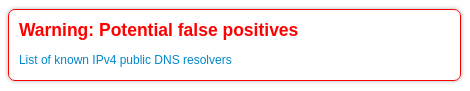
\includegraphics[scale=0.8]{screenshots/false-positive.png}
\end{frame}

\begin{frame}
\frametitle{Managing sub-communities}
\begin{itemize}
    \item Often within a community {\bf smaller bubbles of information sharing will form}
	\item For example: Within a national private sector sharing community, specific community for financial institutions
	\item Sharing groups serve this purpose mainly
	\item As a CSIRT running a national community, consider bootstraping these sharing communities
	\item Organisations can of course self-organise, but you are the ones with the know-how to get them started
\end{itemize}
\end{frame}

\begin{frame}
\frametitle{Managing sub-communities}
\begin{itemize}
	\item Consider compartmentalisation - does it make sense to move a secret squirrel club to their own sharing hub to avoid accidental leaks?
    \item Use your {\bf best judgement} to decide which communities should be separated from one another
    \item Create sharing hubs with {\bf manual data transfer} if needed
	\item Some organisations will even have their data air-gapped - Feed system
    \item {\bf Create guidance} on what should be shared outside of their bubbles - organisations often lack the insight / experience to decide how to get going. Take the initiative!
\end{itemize}
\end{frame}

\begin{frame}
\frametitle{Get in touch if you need some help to get started}
\begin{itemize}
\item Getting started with building a new community can be daunting. Feel free to get in touch with us if you have any questions!
\item Contact: info@circl.lu
\item \url{https://www.circl.lu/}
\item \url{https://github.com/MISP}  \url{https://gitter.im/MISP/MISP}  \url{https://twitter.com/MISPProject}
\end{itemize}
\end{frame}
